\chapter{Introduction}

\section{Motivation}
Sonar (\autoref{sec:sonar}) is an open source software quality platform that uses various static code analysis tools such as Checkstyle, PMD and FindBugs to extract software metrics, which can be used to improve software quality. For source code, Sonar can even give comments on analyzed code, such as what kind of major bugs are found or conventions are not hold and what can be done to resolve it. Usually, Sonar is used in combination with programming languages, like Java, C or C\#, but Sonar indeed gives the functionality to display all kind of measures and handle more than just source code. From model driven software development we know, that all the object oriented ideas also can be mapped to models, which represent the original objects. So in fact, we also could analyze models instead of just source code. This aspect can be very useful in enterprises, which only work model driven. Instead of transforming their models into source code, they can only rely on the standards, given for the used model language, and can analyze their models with Sonar. This has a great advantage: Instead of firstly generating code from their models and then analyzing their source code by Sonar, they simply can use the models only, analyze them with Sonar and only when the measurements reached a specified threshold, they can generate code from their models. Thus, developers can evaluate, change and improve code quality before generating code. 

Modelbus (\autoref{sec:modelbus}) is a model repository, which is used to achieve a seamless integration between tools and the work of the development team. In Modelbus, system information (models) can be stored and reused in a transparent way. Therefore it would be an important feature to analyze models located in such a Modelbus repository.

Since we cannot simply use all of the metrics we know from object oriented code analysis, Sonar cannot be run out of the box to analyze models. Our plugin should therefore use the Metrino service (\autoref{sec:metrino}), which gives us the functionality to examine all of the metrics on models as well. So with our work we want to provide a Sonar plugin to analyze models located at a Modelbus repository using the Metrino Service.

\section{Expectations}
Our team consists of six computer science MSc students who are motivated to find a stable solution for the given task: Alexander Dümont, Arsenij Solovjev, Damla Durmaz, Ferhat Beyaz, Markus Rudolph, Sebastian Barthel.
Our goal is to expand Sonar to cooperate with ModelBus. At the beginning of the course none of us had experience in working with neither Sonar nor Modelbus nor Metrino. So in fact our first expectation was to learn the usage of those software systems. We also had not much experience in the model driven software developement. Therefore it should be necessary to learn to work with models and to generate code from it (as later used with the SMM parser and other software components). Although we had no experience with those systems, their good programming interfaces are promising to work fluently together.

\section{Model-Driven Engineering}
With model-driven engineering we focus on domain models rather then on objects in the sense of object oriented programming. Those domain models are anbstract representations of the knowledge and activities that belong them). We can compare them with objects, but instead of describing them with sourcecode from programming languages like Java or C we simply use UML and generate the sourcecode from it.

With the usage of standardized models model-driven engineering wants to maximize the compatibility between systems and wants to increase the overall productivity. Models are developed in the communication process between the product owner, developers and other people (designers, etc). As the model set approaches completion, developement process can be started.

\section{Requirements}
The product owner presented us their system with Modelbus and the Metrino service. They explained, that in the Modelbus repository, there are models which can be analyzed by the Metrino service and that it can be interesting to get to know in what extend object oriented metrics of Sonar can be applied to models. Therefore, we identified some requirements for our Sonar plugin:
\begin{enumerate}
\item Create a plugin for sonar 
\item Comprehend and cooperate with ModelBus repository
\item Transfer as many as possible metrics from Metrino to Sonar
\item Select the model
\item Traverse the directory tree
\item Analyze source codes
\item Plugin must work as efficient as possible
\end{enumerate}
In the following sections, the requirements will be described in detail and are divided into functional and non-functional requirements.

\subsection{Functional requirements}

\begin{table}[H]
\begin{tabular}{|c|p{10cm}|}
\hline 
\multicolumn{2}{|l|}{\textbf{Create a plugin for Sonar}} \\ 
\hline 
Requirement Number & 1 \\ \hline 
Description & Each sonar plugin has a specific architecture. The created sonar plugin must hold the specifications for a sonar plugin. Additionally, it must be run on a server and offers a WSDL interface. \\ \hline 
Dependencies & \textbf{none} (should be done first) \\ \hline 
Priority & high \\ \hline 
State & closed \\ \hline 
Fit Criterion & The plugin can be build and runs on a chosen server. A client connects to the Modelbus server and understands the WSDL interface. The client receives a message from the WSDL interface of the Modelbus server. \\ \hline 
\end{tabular}
\end{table}

\begin{table}[H]
\begin{tabular}{|c|p{10cm}|}
\hline 
\multicolumn{2}{|l|}{\textbf{Comprehend and cooperate with ModelBus repository}} \\ 
\hline 
Requirement Number & 2 \\ \hline 
Description & ModelBus has an own repository, where it stores artifacts of the tools, which are connected to the ModelBus via adapters. It must be understood, how ModelBus connects to the repository and how an external tool (like a sonar plugin) can do this. \\ \hline 
Dependencies & \# 1 \\ \hline 
Priority & high \\ \hline 
State & closed \\ \hline 
Fit Criterion & The sonar plugin is able to connect to the ModelBus repository via a command. It can fetch the source code for a random project to test, if the connection is established. The sonar plugin can terminate the connection to the repository for a given command. \\ \hline 
\end{tabular}
\end{table}

\begin{table}[H]
\begin{tabular}{|c|p{10cm}|}
\hline 
\multicolumn{2}{|l|}{\textbf{Select the model}} \\ 
\hline 
Requirement Number & 4 \\ \hline 
Description & The sonar plugin can fetch model code from the repository and transform the model into a format which can be read by model metric analyzing tools, like Metrino. \\ \hline 
Dependencies & \# 3 \\ \hline 
Priority & high \\ \hline 
State & closed \\ \hline 
Fit Criterion & The plugin fetched a model. It transforms the model into the format of Metrino. For a test case, the transformed model shall be saved in a file and read successfully by Metrino. \\ \hline 
\end{tabular}
\end{table}
\vspace{-30mm}
\begin{table}[H]
\begin{tabular}{|c|p{10cm}|}
\hline 
\multicolumn{2}{|l|}{\textbf{Traverse the directory tree}} \\ 
\hline 
Requirement Number & 5 \\ \hline 
Description & In the directory tree of sonar plugin, a lot of source code and model code projects are placed. The plugin should be able to analyze all codes from the repository. \\ \hline 
Dependencies & \textbf{none} \\ \hline 
Priority & high \\ \hline 
State & closed \\ \hline 
Fit Criterion & The plugin fetched the whole project tree of the repository. It loads each project into its own directory tree. It traverses the whole directory tree. For each project in its directory tree, it analyzes the code and visualizes it on the web interface. \\ \hline 
\end{tabular}
\end{table}

\noindent\begin{minipage}{\linewidth}
\centering
\begin{tabular}{|c|p{10cm}|}
\hline 
\multicolumn{2}{|l|}{\textbf{Analyze source codes}} \\ 
\hline 
Requirement Number & 6 \\ \hline 
Description & The sonar plugin can apply a set of metrics to the fetched source code. The results are visualized with graphs or statistics and can be get via the web interface. \\ \hline 
Dependencies & \# 2 \\ \hline 
Priority & high \\ \hline 
State & Canceled, because requirement is unfeasible with current Sonar version (could be with future versions) \\ \hline 
Fit Criterion & The plugin fetches source code from the repository. It applies a couple of metrics, which can be chosen from the application interface. \\ \hline 
\end{tabular}
\end{minipage}

\subsection{Non-functional requirements}

\noindent\begin{minipage}{\linewidth}
\centering
\begin{tabular}{|c|p{10cm}|}
\hline 
\multicolumn{2}{|l|}{\textbf{Transfer as many as possible metrics from Metrino to Sonar}} \\ 
\hline 
Requirement Number & 3 \\ \hline 
Description & The sonar plugin can already fetch model code from the repository. The models are read by Metrino and analyzed by Metrino with object oriented metrics. The results of the analysis are fetched from Metrino by the sonar plugin and visualized on the web interface. Metrino offers a lot of metrics and it should be possible to offer as many metrics from Metrino as possible. \\ \hline 
Dependencies & \# 4 \\ \hline 
Priority & high \\ \hline 
State & open \\ \hline 
Fit Criterion & The sonar plugin sends a model to Metrino with the information which object oriented metric shall be applied. Metrino returns the results. The results are visualized. The plugin offers to select at least $10$ object oriented metrics of Metrino to apply to the sent model code. \\ \hline 
\end{tabular}
\end{minipage}

\noindent\begin{minipage}{\linewidth}
\centering
\begin{tabular}{|c|p{10cm}|}
\hline 
\multicolumn{2}{|l|}{\textbf{Plugin must work as efficient as possible}} \\ 
\hline 
Requirement Number & 7 \\ \hline 
Description & Plugin must traverse the directory tree fastly. The connection to the ModelBus must provide security standards, but it should not be slow. The results of the analysis should be offerred via the web interface as fast as possible. \\ \hline 
Dependencies & \# 6 \\ \hline 
Priority & middle \\ \hline 
State & closed \\ \hline 
Fit Criterion & Because of the difficulty of the decision, if it works properly fast, a usability test with the customer must be done, who can tell in a better way, if the product works fast or not. \\ \hline 
\end{tabular}
\end{minipage}



\section{Responsibilities and Progress}
\begin{table}[htbp]
  \caption{Exercises pt. 1}
  \noindent\hspace*{-1cm}\begin{tabularx}{\textwidth+2cm}{
>{\raggedleft\arraybackslash\advance\hsize1em}X
>{\raggedright\arraybackslash\advance\hsize1em }X
>{\raggedright\arraybackslash}X
>{\raggedright\arraybackslash\advance\hsize-1em }X
>{\raggedright\arraybackslash\advance\hsize-1em }X
}
    \addlinespace
    \toprule
    \multicolumn{1}{c}{Exercise } & Begin & End  & Progress & Done by   \\
    \midrule
         
        Explore Modelbus & Mo 05.11.12 & Fr 09.11.12 & 100\% & Team \\
Explore Sonar                                                           & Mo 05.11.12 & Fr 09.11.12 & 100\%     & Team                    \\ 
        Explore plugin developement possibilities                               & Mo 05.11.12 & Fr 09.11.12 & 100\%     & Ferhat                  \\ 
        Explore Sonar features and developement possibilities                   & Mo 05.11.12 & Fr 09.11.12 & 100\%     & Damla                   \\ 
        First attempt to plugin developement                                    & Mo 05.11.12 & Fr 09.11.12 & 100\%     & Markus                  \\ 
        Wiki Introduction                                                       & Mo 05.11.12 & Fr 09.11.12 & 100\%     & Sebastian               \\ 
        Modelbus connection                                                     & Mo 05.11.12 & Fr 09.11.12 & 100\%     & Arsenij                 \\ 
        Sonar documentation                                                     & Mo 05.11.12 & Fr 09.11.12 & 100\%     & Markus                  \\ 
        Wiki Metrino                                                            & Mo 05.11.12 & Fr 09.11.12 & 100\%     & Alexander               \\ 
        Sonar plugin documentation                                              & Mo 05.11.12 & Fr 09.11.12 & 100\%     & Ferhat                  \\ 
        Modelbus documentation                                                  & Mo 05.11.12 & Fr 09.11.12 & 100\%     & Damla                   \\ 
        Requirements                                                            & Mo 05.11.12 & Fr 09.11.12 & 100\%     & Damla  \&  Ferhat       \\ 
        Presentation Requirements                                               & Mo 05.11.12 & Fr 09.11.12 & 100\%     & Ferhat                  \\ 
        Improve requirements                                                    & Mo 12.11.12 & Fr 16.11.12 & 100\%     & Damla                   \\ 
        \hline
    \end{tabularx}\hspace*{-1cm}%
  \label{tab:addlabel}%
\end{table}%

\begin{table}[htbp]
  \caption{Exercises pt. 2}
  \noindent\hspace*{-1cm}\begin{tabularx}{\textwidth+2cm}{
>{\raggedleft\arraybackslash\advance\hsize1em}X
>{\raggedright\arraybackslash\advance\hsize1em }X
>{\raggedright\arraybackslash}X
>{\raggedright\arraybackslash\advance\hsize-1em }X
>{\raggedright\arraybackslash\advance\hsize-1em }X
}
    \addlinespace
    \toprule
    \multicolumn{1}{c}{Exercise } & Begin & End  & Progress & Done by   \\
    \midrule
        Architecture conecept for sonar                                         & Mo 12.11.12 & Fr 16.11.12 & 100\%     & Ferhat                  \\ 
        Architecture conecept for metrino                                       & Mo 12.11.12 & Fr 16.11.12 & 100\%     & Alexander               \\ 
        Introduction to wiki                                                    & Mo 12.11.12 & Mo 19.11.12 & 100\%     & Sebastian               \\ 
        Presentation Template                                                   & Mo 12.11.12 & Fr 19.11.12 & 100\%     & Damla                   \\ 
        Software architecture – sequencediagram/activitydiagram                 & Mo 12.11.12 & Fr 23.11.12 & 100\%     & Sebastian               \\ 
        Setup Modelbus Repository Server                                        & Mo 19.11.12 & Mo 26.11.12 & 100\%     & Arsenij                 \\ 
        Explore howto running sonar on a repository                             & Di 20.11.12 & Mo 26.11.12 & 100\%     & Arsenij                 \\ 
        Installation of software components                                     & Do 23.11.12 & Do 23.11.12 & 100\%     & Team                    \\ 
        Example Sonar plugin                                                    & Mo 19.11.12 & Fr 23.11.12 & 100\%     & Unknown                 \\ 
        Multilanguage (different programming languages) support in sonar plugins & Fr 23.11.12 & Do 29.11.12 & 100\%     & Markus  \&  Damla  \&  Ferhat \\ 

        \hline
    \end{tabularx}\hspace*{-1cm}%
  \label{tab:addlabel}%
\end{table}%

\begin{table}[htbp]
  \caption{Exercises pt. 3}
  \noindent\hspace*{-1cm}\begin{tabularx}{\textwidth+2cm}{
>{\raggedleft\arraybackslash\advance\hsize1em}X
>{\raggedright\arraybackslash\advance\hsize1em }X
>{\raggedright\arraybackslash}X
>{\raggedright\arraybackslash\advance\hsize-1em }X
>{\raggedright\arraybackslash\advance\hsize-1em }X
}
    \addlinespace
    \toprule
    \multicolumn{1}{c}{Exercise } & Begin & End  & Progress & Done by   \\
    \midrule
        Sequence diagram for the work of sonar with Metrino and ModelBus        & So 25.11.12 & So 25.11.12 & 100\%     & Damla  \&  Sebastian    \\ 
        Setup modelbus server                                                   & Fr 23.11.12 & Mo 26.11.12 & 100\%     & Markus                  \\ 
        Presentation first architecture                                         & Fr 23.11.12 & Mo 26.11.12 & 100\%     & Ferhat                  \\ 
        Activity diagram modelbus repository                                    & Fr 23.11.12 & Mo 26.11.12 & 100\%     & Damla                   \\ 
        SOAP Client Metrino                                                     & Fr 23.11.12 & Do 06.12.12 & 100\%     & Alexander               \\ 
        Wiki Logo and header                                                    & Mo 26.11.12 & Fr 30.11.12 & 100\%     & Ferhat                  \\ 
        OCL  \&  Documentation                                                  & Mo 26.11.12 & Fr 30.11.12 & 100\%     & Damla  \&  Ferhat       \\ 
        Milestone definitions and description                                   & Mo 26.11.12 & Fr 30.11.12 & 100\%     & Sebastian               \\ 
        Installation manual                                                     & Mo 03.12.12 & Mo 10.12.12 & 100\%     & Sebastian               \\ 
        Include other language plugins with modules                             & Mo 03.12.12 & Mo 10.12.12 & 100\%     & Arsenij                 \\ 
        \hline
    \end{tabularx}\hspace*{-1cm}%
  \label{tab:addlabel}%
\end{table}%


\begin{table}[htbp]
  \caption{Exercises pt. 4}
  \noindent\hspace*{-1cm}\begin{tabularx}{\textwidth+2cm}{
>{\raggedleft\arraybackslash\advance\hsize1em}X
>{\raggedright\arraybackslash\advance\hsize1em }X
>{\raggedright\arraybackslash}X
>{\raggedright\arraybackslash\advance\hsize-1em }X
>{\raggedright\arraybackslash\advance\hsize-1em }X
}
    \addlinespace
    \toprule
    \multicolumn{1}{c}{Exercise } & Begin & End  & Progress & Done by   \\
    \midrule
        Client without using WSDL by hand                                       & Mo 03.12.12 & Mo 10.12.12 & 100\%     & Markus                  \\ 
        Objectoriented Analysis to Models                                       & Mo 03.12.12 & Mo 10.12.12 & 100\%     & Ferhat                  \\ 
        Understand Metrino metrcis                                              & Mo 10.12.12 & Fr 21.12.12 & 100\%     & Sebastian  \&  Alexander \\ 
        ownload modelbus files in a sonar plugin                                & Mo 10.12.12 & Fr 21.12.12 & 100\%     & Markus                  \\ 
        Create latex documentation                                              & Mo 17.12.12 & Fr 21.12.12 & 100\%     & Ferhat                  \\ 
        Meeting Protocols to latex documentation                                & Mo 17.12.12 & Fr 21.12.12 & 100\%     & Damla                   \\ 
        Metrino CheckModel, download and parse SMM from Repo                    & Mo 07.01.13 & Mo 21.01.13 & 100\%     & Arsenij                 \\ 
        Sonar frontend                                                          & Mo 07.01.13 & Mo 21.01.13 & 100\%     & Sebastian               \\ 
        Parser for SMM                                                          & Mo 14.01.13 & So 20.01.13 & 100\%     & Damla  \&  Ferhat       \\ 
        Using of EMF to parse SMM files                                         & Mo 21.01.13 & Mo 28.01.13 & 100\%     & Damla  \&  Ferhat       \\ 

        \hline
    \end{tabularx}\hspace*{-1cm}%
  \label{tab:addlabel}%
\end{table}%


\begin{table}[htbp]
  \caption{Exercises pt. 5}
  \noindent\hspace*{-1cm}\begin{tabularx}{\textwidth+2cm}{
>{\raggedleft\arraybackslash\advance\hsize1em}X
>{\raggedright\arraybackslash\advance\hsize1em }X
>{\raggedright\arraybackslash}X
>{\raggedright\arraybackslash\advance\hsize-1em }X
>{\raggedright\arraybackslash\advance\hsize-1em }X
}
    \addlinespace
    \toprule
    \multicolumn{1}{c}{Exercise } & Begin & End  & Progress & Done by   \\
    \midrule
        Include parser into project workflow                                    & Mo 21.01.13 & Mo 28.01.13 & 100\%     & Damla  \&  Ferhat       \\ 
        Merge all components into one                                           & Mo 21.01.13 & Mo 28.01.13 & 100\%     & Arsenij                 \\ 
        Project spezific measurements in sonar                                  & Mo 21.01.13 & Mo 28.01.13 & 100\%     & Markus                  \\ 
        ceate ocl metrics                                                       & Mo 21.01.13 & So 03.02.13 & 100\%     & Alexander               \\ 
        Color Measurements                                                      & Mo 21.01.13 & Mo 28.01.13 & 100\%     & Sebastian               \\ 
        Documentation in Latex                                                  & Mo 28.01.13 & Mo 18.02.13 & 25\%      & Team                    \\ 
        SMM Adapter                                                             & Mo 28.01.13 & Mo 18.02.13 & 67\%      & Arsenij                 \\ 
        Load dynamic metrics in sonar                                           & Mo 28.01.13 & Mo 18.02.13 & 36\%      & Sebastian               \\ 
        Meeting Protocols                                                       & Mo 03.12.12 & Mo 18.02.13 & 95\%      & Damla  \&  Ferhat       \\
        
        \hline
    \end{tabularx}\hspace*{-1cm}%
  \label{tab:addlabel}%
\end{table}%

\newpage

\begin{figure}[htb]
\begin{center}
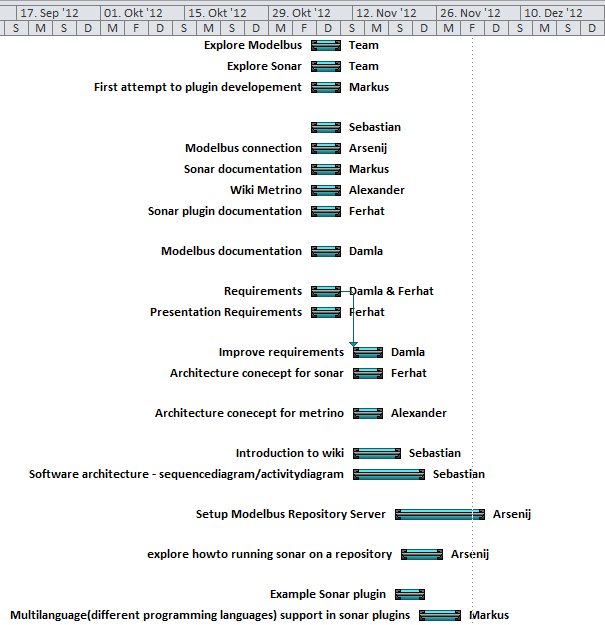
\includegraphics[width=\textwidth]{msp_part1}
\caption{Exercises - MS Project screenshot 1}
\end{center}
\end{figure}

\newpage

\begin{figure}[htb]
\begin{center}
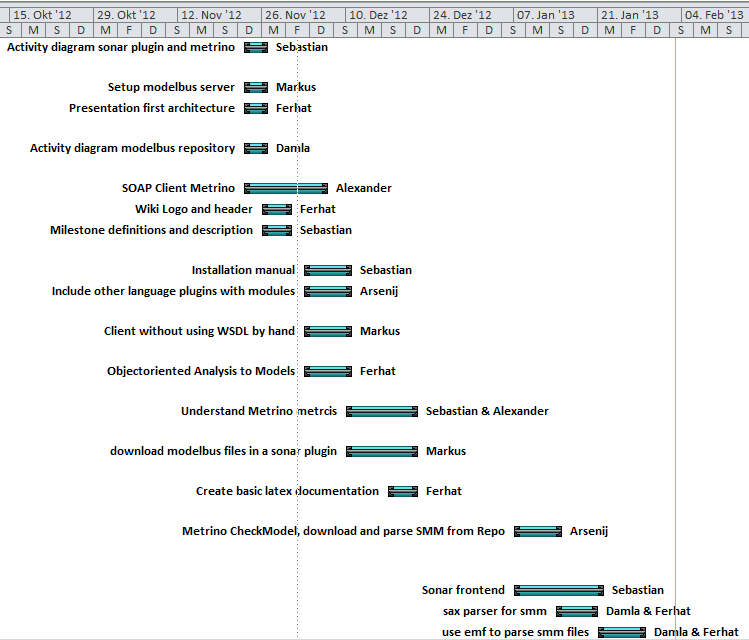
\includegraphics[width=\textwidth]{msp_part2}
\caption{Exercises - MS Project screenshot 2}
\end{center}
\end{figure}

\newpage

\begin{figure}[htb]
\begin{center}
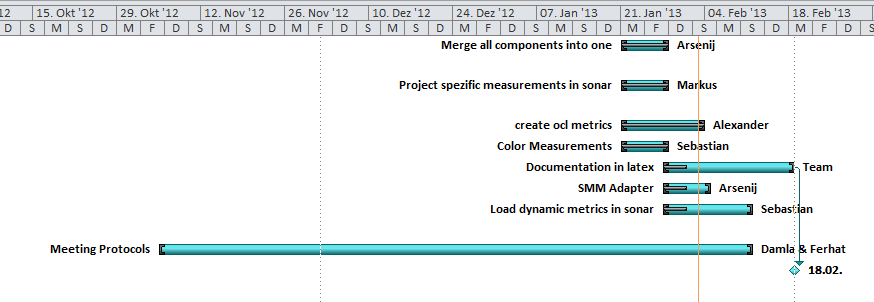
\includegraphics[width=\textwidth]{msp_part3}
\caption{Exercises - MS Project screenshot 3}
\end{center}
\end{figure}

\section{Paper Purposes}
